%
%      Introduction into UML, Principles of Object Oriented Design
%
\section{Part \partNo\ Learning Objectives}

\begin{frame}{What are you about to learn?}
   \begin{block}{Knowledge}
       \begin{itemize}
           \item What is architecture?
           \item Architectural objectives in software design
           \item UML structural modeling elements 
   \end{itemize}
   \end{block}
   \begin{block}{Skills}
       \begin{itemize}
           \item Can detect violations of object oriented design principles
           \item Can explain all object oriented design principles using UML diagrams
   \end{itemize}
\end{block}
\end{frame}

%-------------------------------------------------------------------
\section{What is Architecture?}

\begin{frame}[fragile]{The Parthenon in Athens, Greece}
\begin{center}
  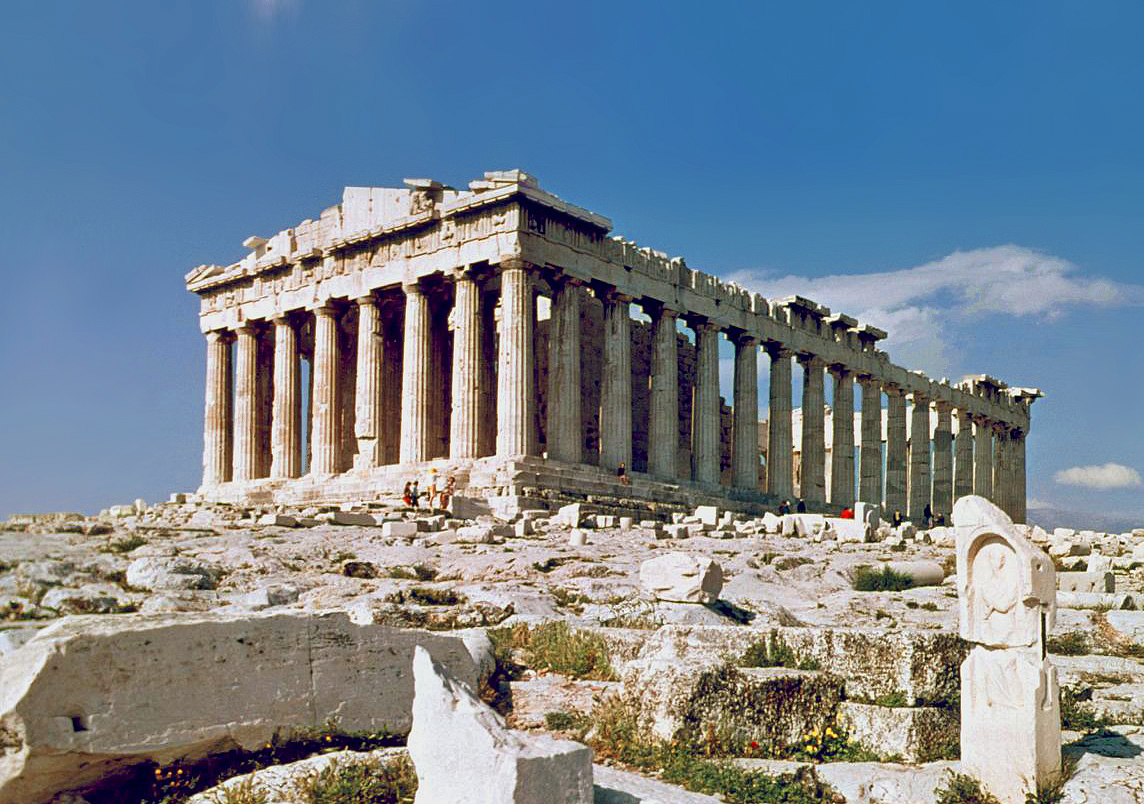
\includegraphics[height=180pt]{partenon.jpg}
\end{center}
\end{frame}

\begin{frame}[fragile]{Some Genius Improvising}
\begin{center}
  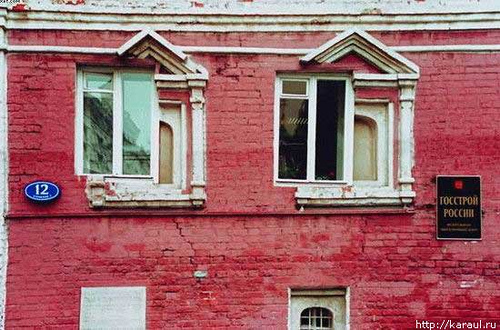
\includegraphics[height=180pt]{badbuilding1.jpg}
\end{center}
\end{frame}

\begin{frame}[fragile]{The Houses of Parliament, London}
\begin{center}
  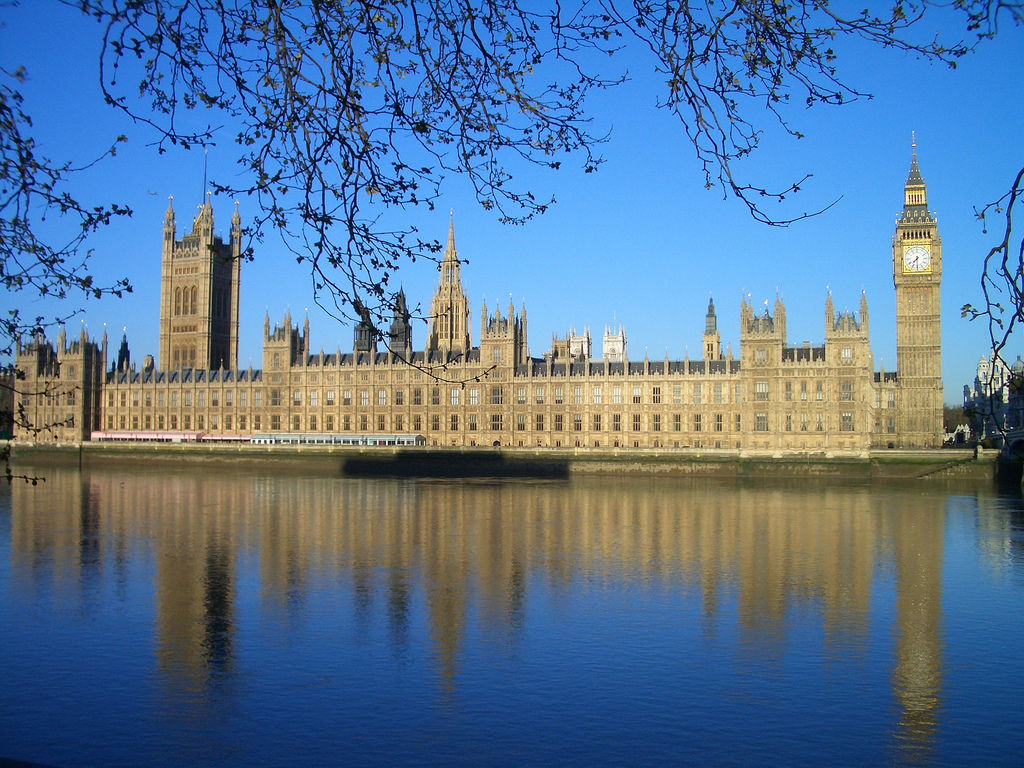
\includegraphics[height=180pt]{Westminster.jpg}
\end{center}
\end{frame}

\begin{frame}[fragile]{The Bauhaus in Dessau, Germany}
\begin{center}
  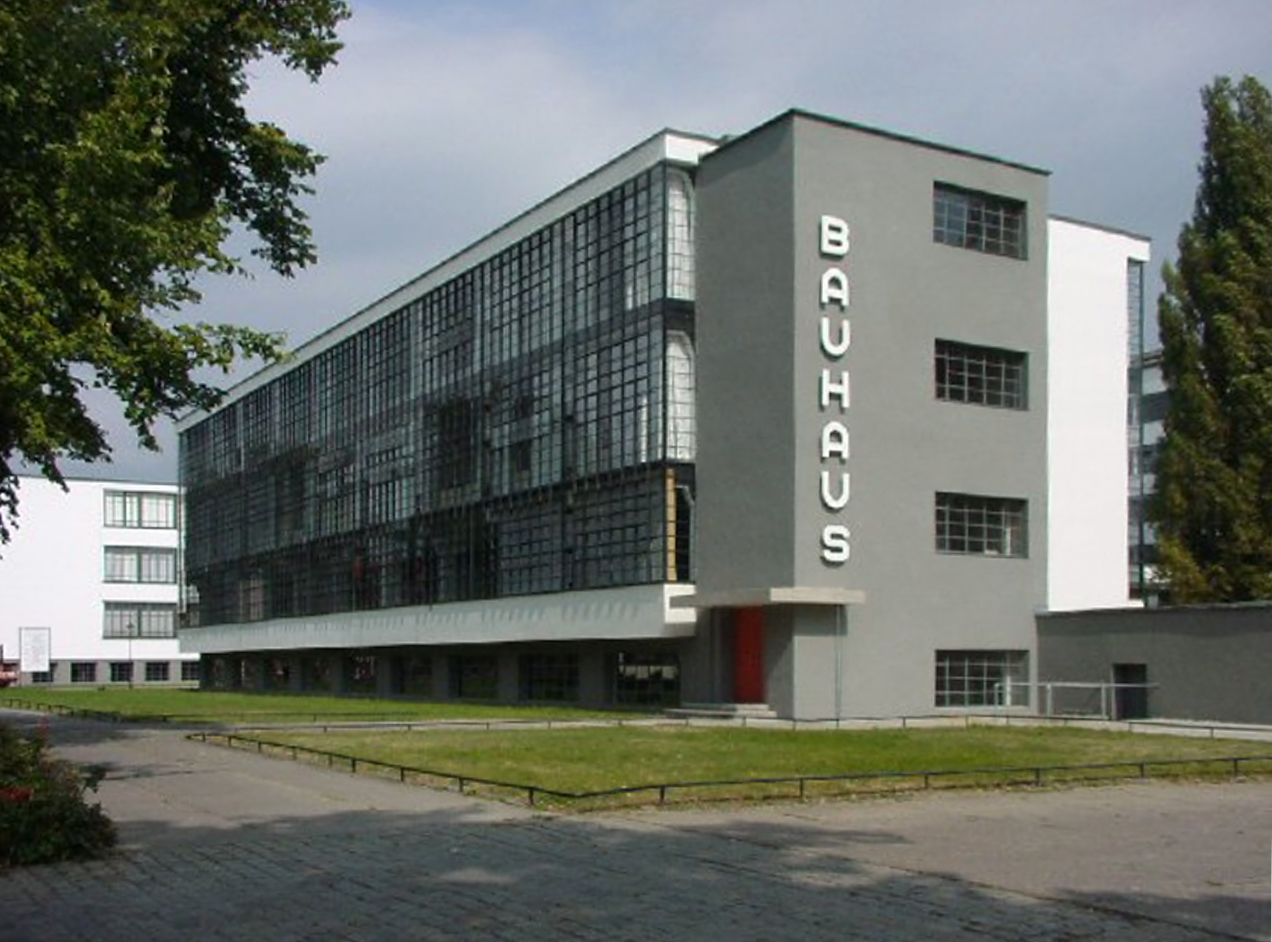
\includegraphics[height=180pt]{Bauhaus.jpg}
\end{center}
\end{frame}

\begin{frame}[fragile]{The Taj Mahal, India}
\begin{center}
  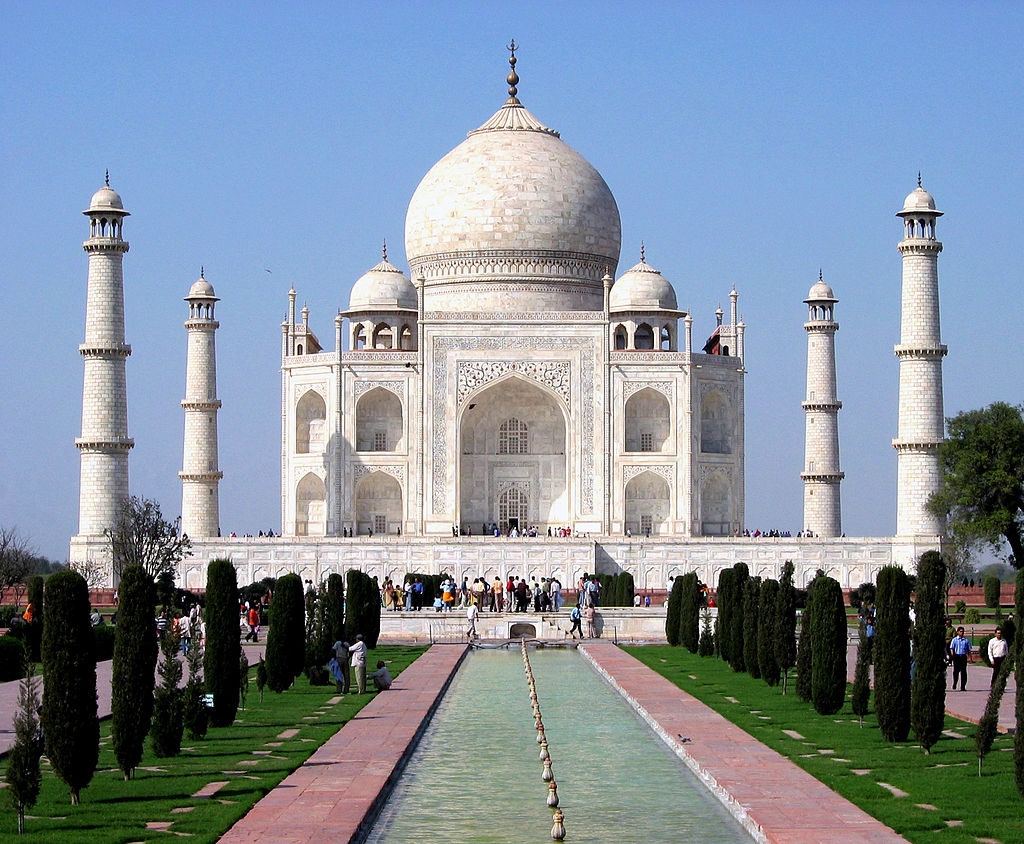
\includegraphics[height=180pt]{TajMahal.jpg}
\end{center}
\end{frame}

\begin{frame}[fragile]{The National Congress of Brazil}
\begin{center}
  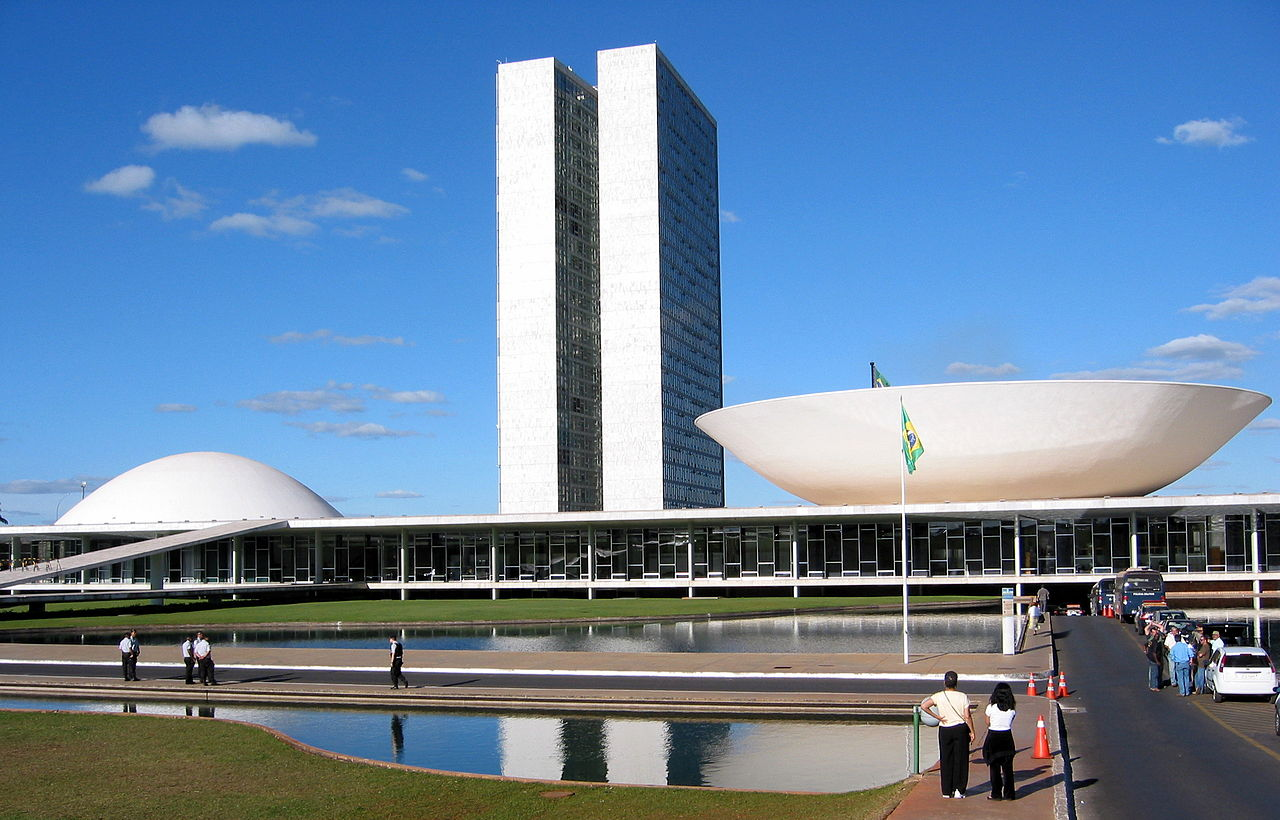
\includegraphics[height=180pt]{CongressoDoBrasil.jpg}
\end{center}
\end{frame}

\begin{frame}[fragile]{The Carpenter did the Design}
\begin{center}
  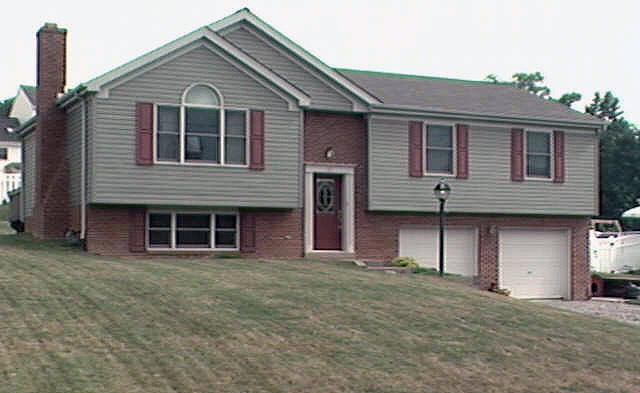
\includegraphics[height=180pt]{badbuilding2.jpg}
\end{center}
\end{frame}

\begin{frame}[fragile]{The Gare de Oriente in Lisbon, Portugal}
\begin{center}
  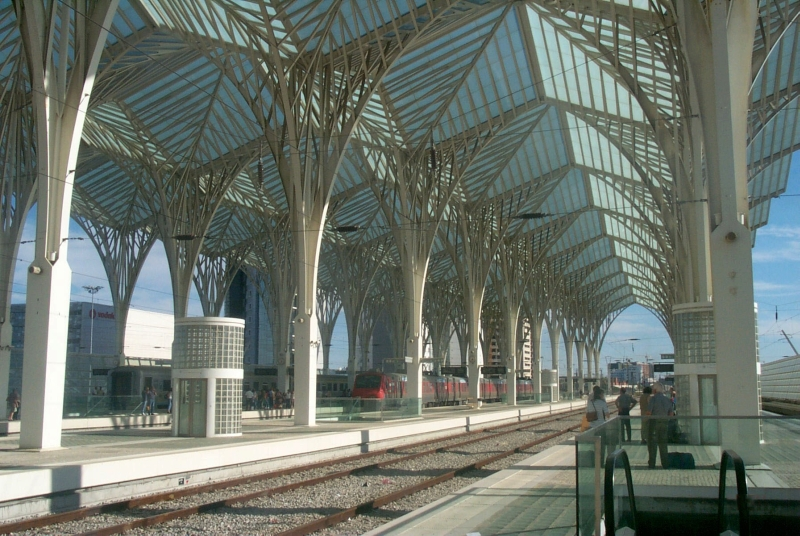
\includegraphics[height=180pt]{OrienteStationLisboa.jpg}
\end{center}
\end{frame}

\begin{frame}[fragile]{The Golden Pavilion in Kyoto, Japan}
\begin{center}
  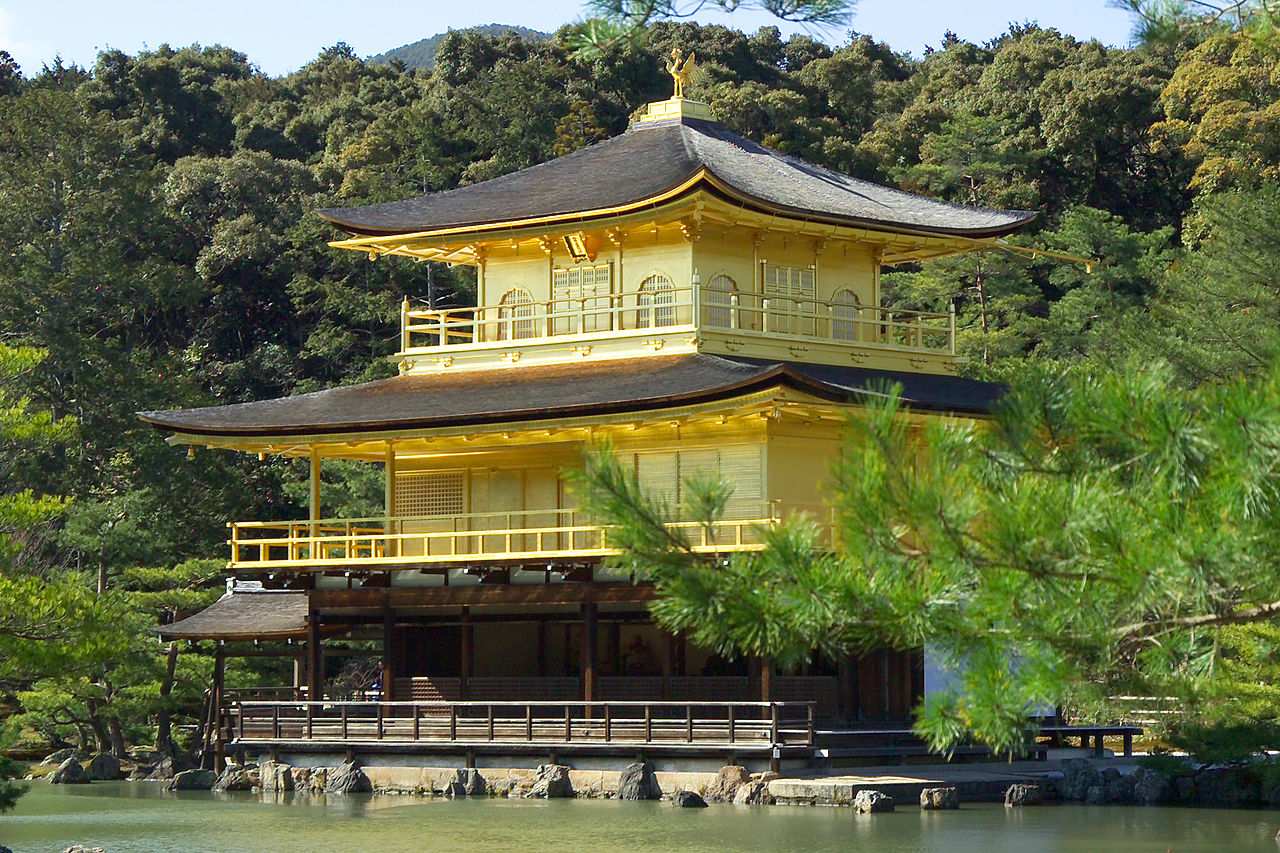
\includegraphics[height=180pt]{Kinkaku.jpg}
\end{center}
\end{frame}

\begin{frame}[fragile]{Notre Dame de Paris, France}
\begin{center}
  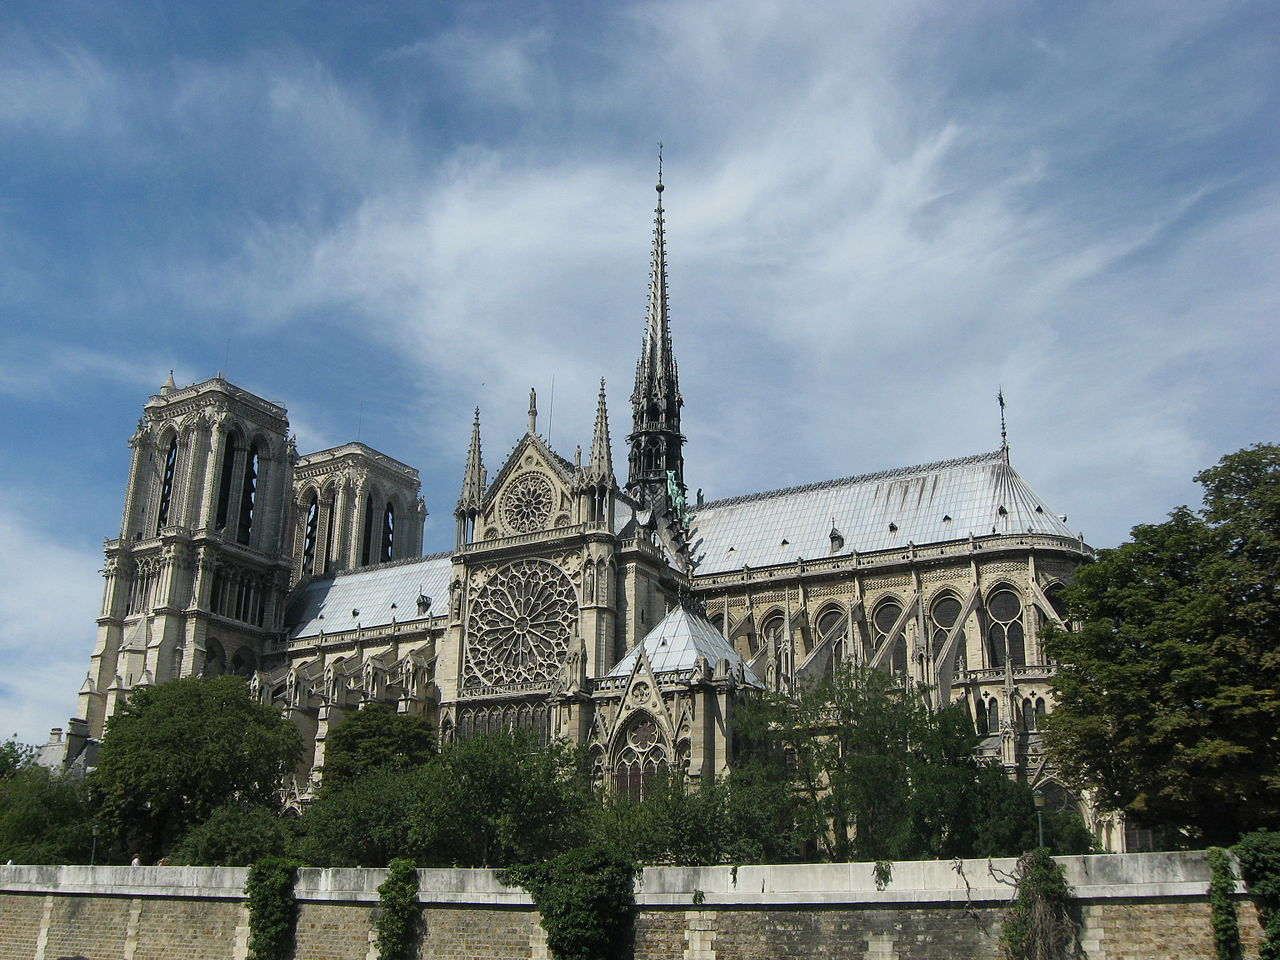
\includegraphics[height=180pt]{NotredameParis.jpg}
\end{center}
\end{frame}

\begin{frame}[fragile]{MI6 Headquarter in London}
\begin{center}
  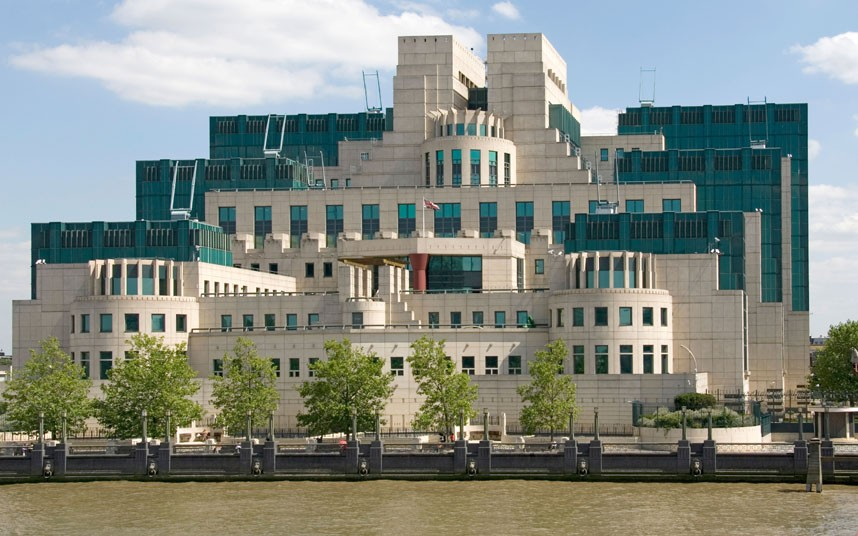
\includegraphics[height=180pt]{mi6.jpg}
\end{center}
\end{frame}

\begin{frame}[fragile]{Shantytown, New Orleans}
\begin{center}
  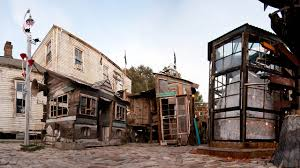
\includegraphics[height=180pt]{badbuilding3.jpg}
\end{center}
\end{frame}

\begin{frame}[fragile]{The Opera House in Sydney, Australia}
\begin{center}
  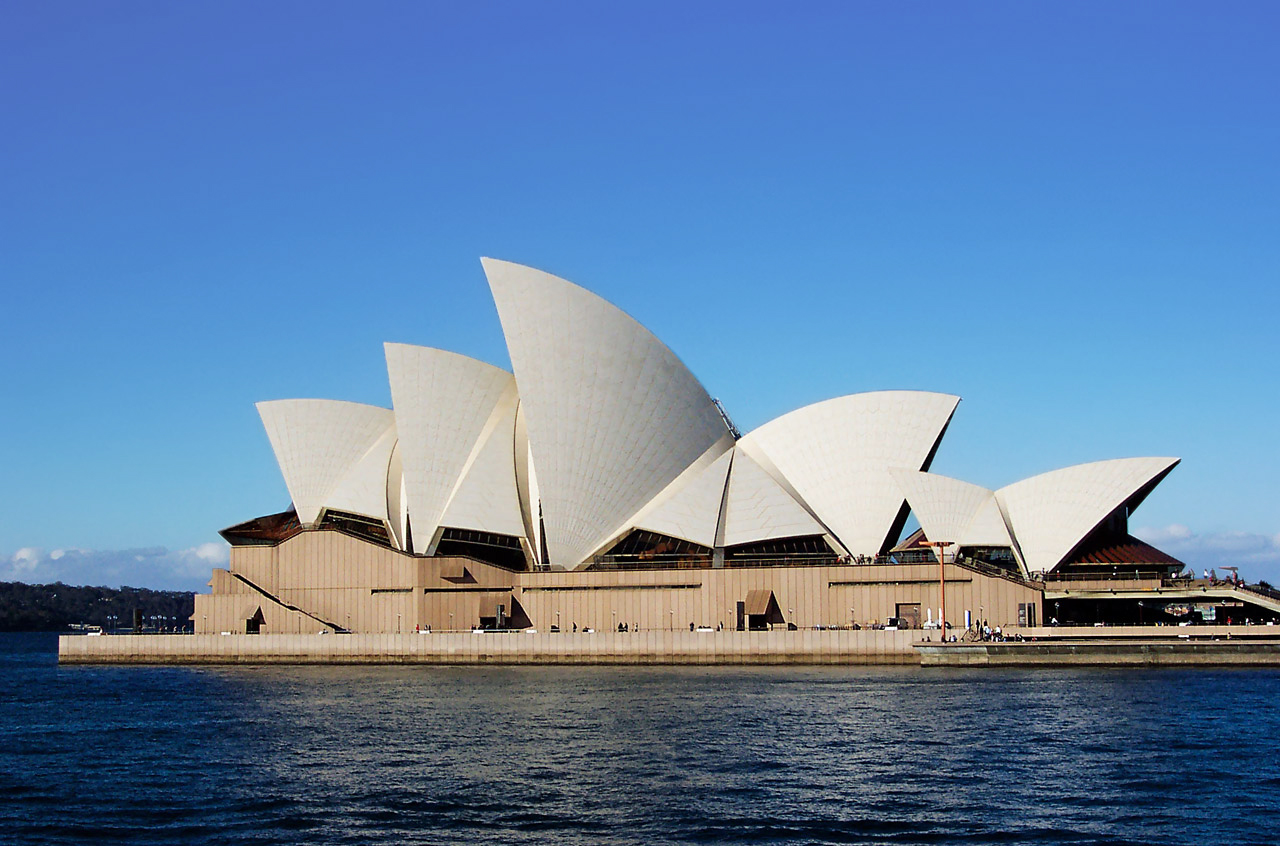
\includegraphics[height=180pt]{SydneyOpera.jpg}
\end{center}
\end{frame}

\begin{frame}{What is Architecture?}
   \begin{block}{Architecture}
       \begin{itemize}
           \item A general term to describe buildings and other physical and some non-physical structures.
           \item The art and science of designing buildings and (some) nonbuilding structures ("Baukunst").
           \item The style of design and method of construction of buildings and other physical and non-physical structures.
   \end{itemize}
\end{block}

   Architecture has to consider
   \begin{itemize}
      \item functional
      \item technical
      \item aesthetic
   \end{itemize}
   aspects in the planning, designing, and construction of its artefacts.
\end{frame}


%-------------------------------------------------------------------
\section{Describing Architecture}


%-------
\begin{frame}{Talking about Things}
      We use \glspl{model} to describe \emph{things} in the real world. 

  \vspace*{1ex}
  Models are abstractions of the real world, simplifying reality.
  
\vspace*{1ex}
   Models describe 
   \begin{itemize}
      \item \Gls{structure}
      \item \Gls{behaviour}
   \end{itemize}

  \vspace*{1ex} 
   Examples
   \begin{itemize}
      \item Buildings (structure)
      \item Elevators (structure and behaviour)
      \item Buying something from an online-shop (behaviour)
      \item Cars (structure and behaviour)
   \end{itemize}
  
\end{frame}

%--------
\begin{frame}{Architecture: Talking about Structure}
   Describing architecture we focus on \gls{structure}.

   For software systems we use the \gls{umll} (\gls{UML}).

\begin{center}
  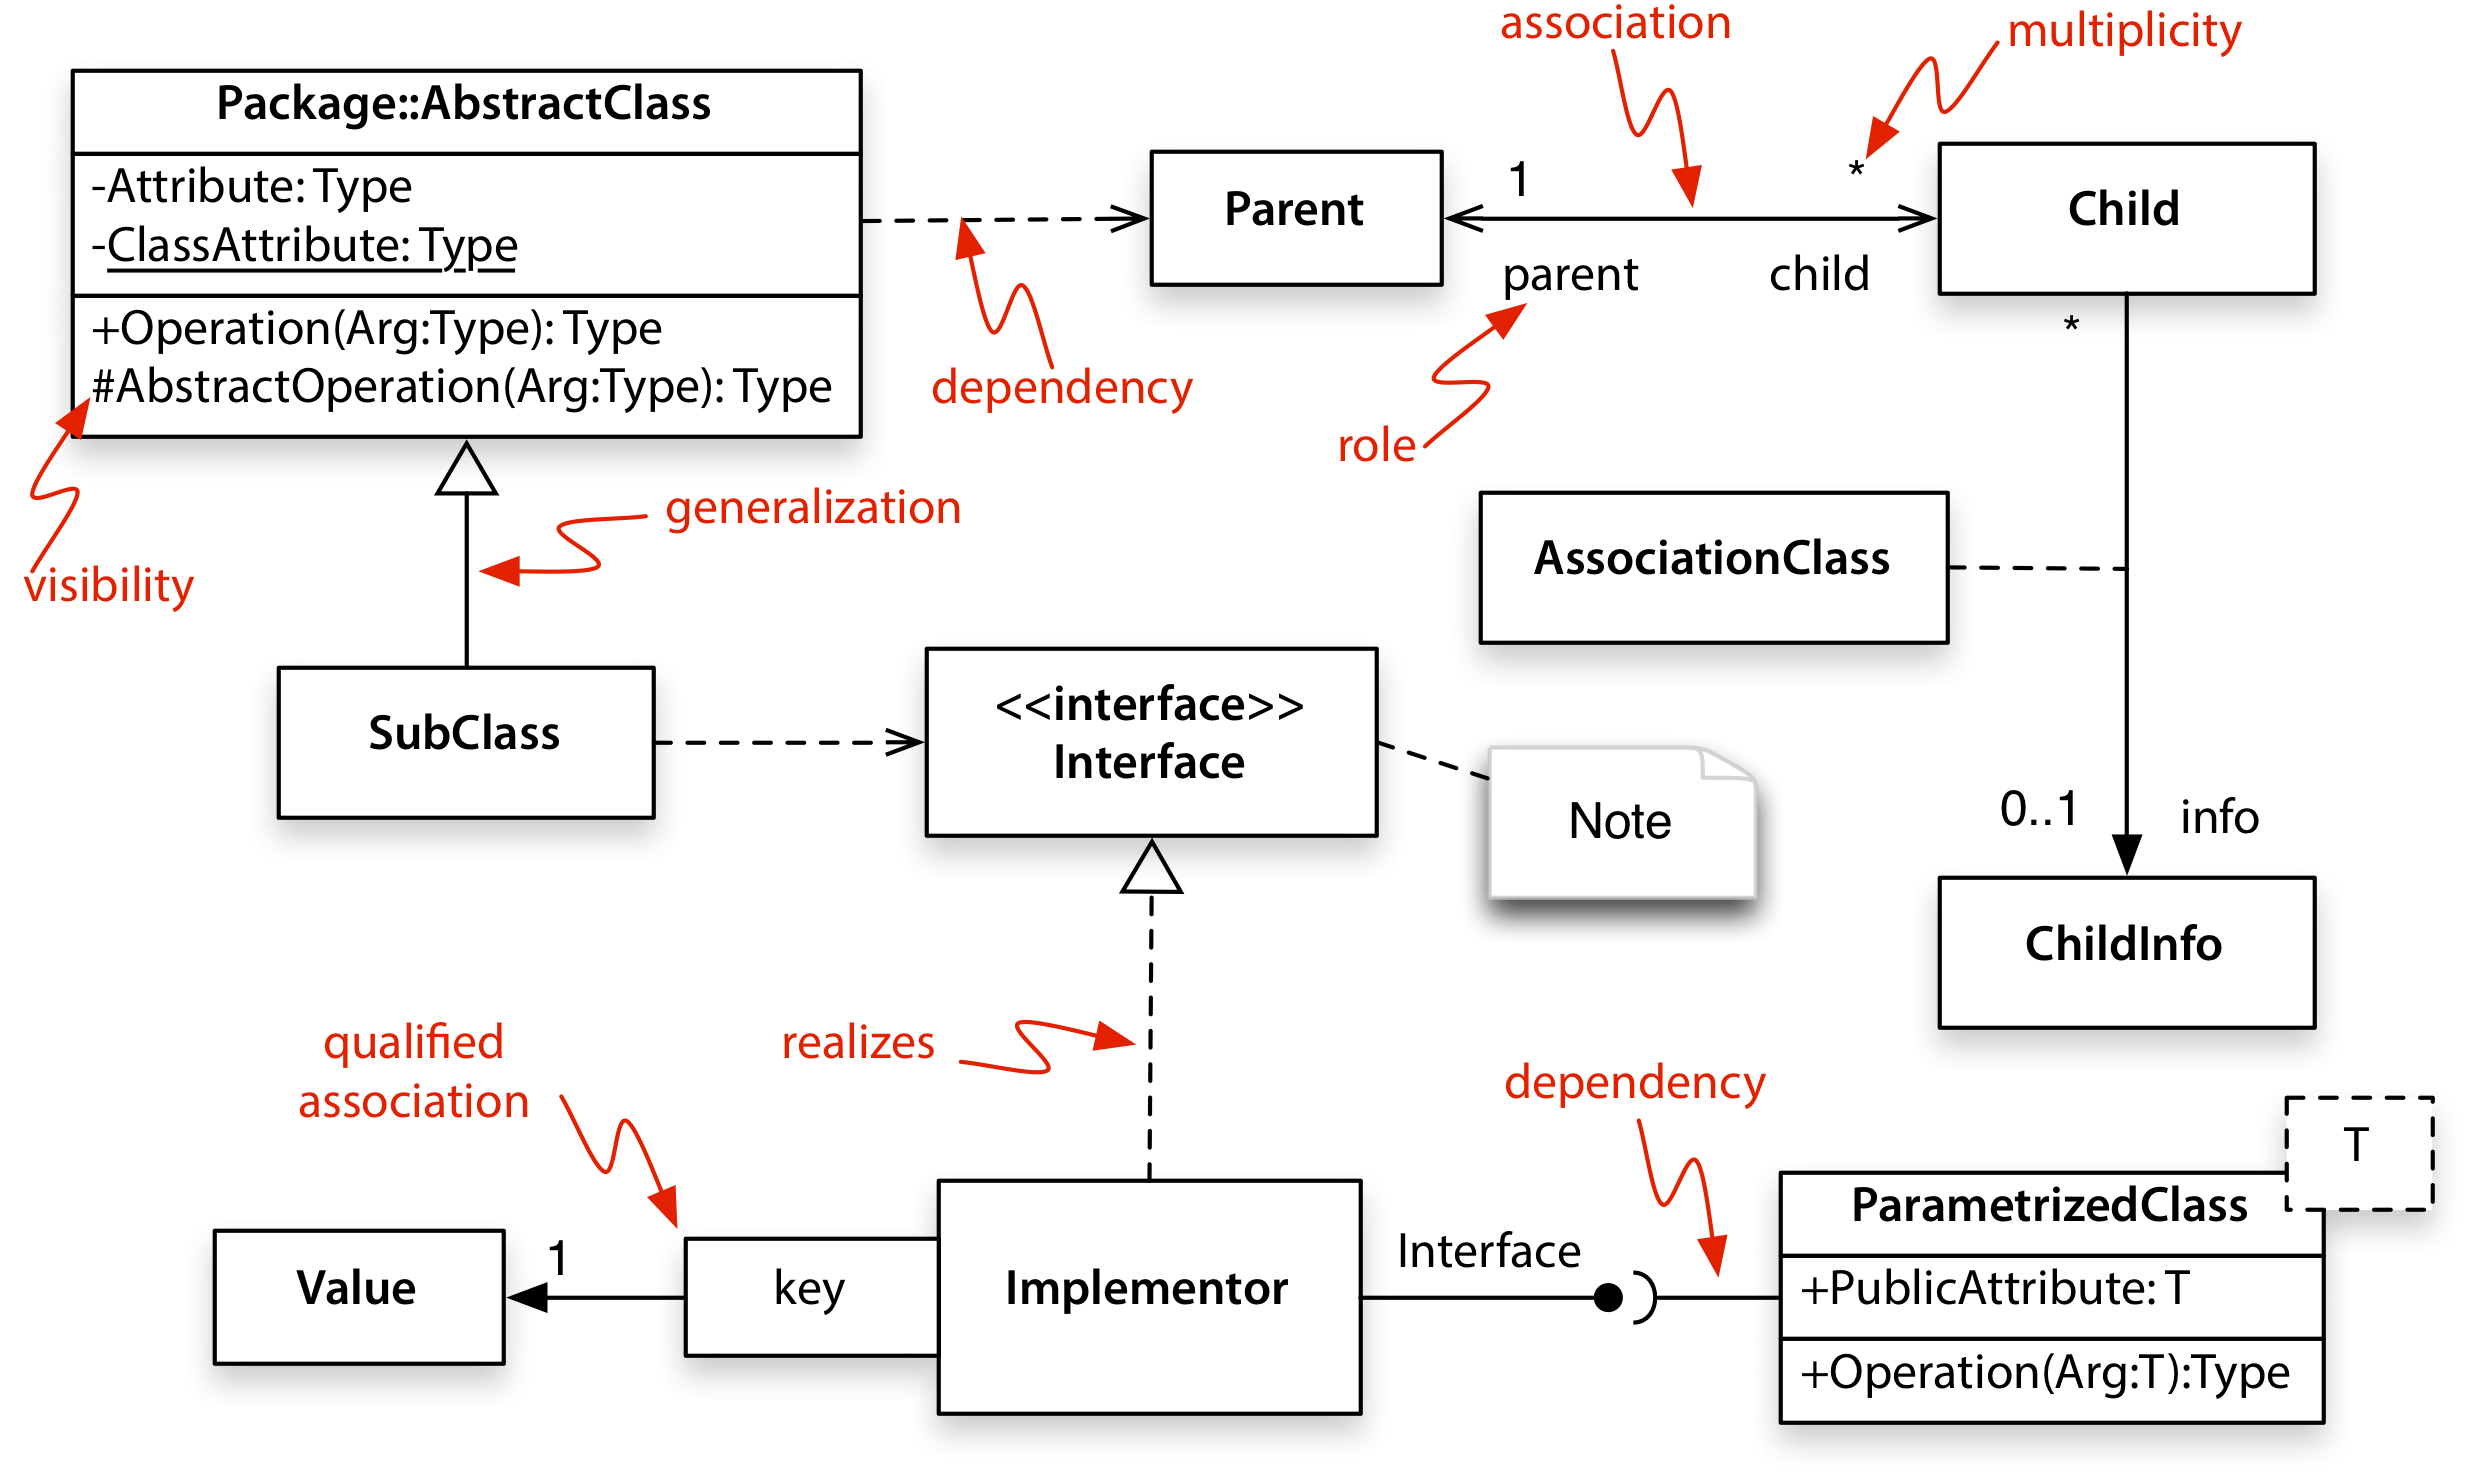
\includegraphics[height=180pt]{umlclasscheat.png}
\end{center}
  
\end{frame}

%--------
\begin{frame}{UML Overview}
The UML offers a rich set of diagram types to describe structure and behaviour.
    \begin{itemize}
       \item \textbf{\color{blue}Class diagrams} {\color{red}$\leftarrow$ this is what we use here}
      \item Component diagrams
       \item Activity diagrams {\color{red}$\leftarrow$ covered in "Real-Time Systems"}
       \item State charts  {\color{red}$\leftarrow$ covered in "Real-Time Systems"}
        \item Sequence diagrams
        \item Use case diagrams
         \item and eight more ...
   \end{itemize}
\end{frame}


%--------
\begin{frame}{Class Diagram: Overview}
    \begin{itemize}
       \item \Glspl{attribute} describe the appearance and knowledge of a class of objects.
       \item \Glspl{operation} define the behavior that a class of objects can manifest.
       \item \Glspl{stereotype} help you understand this type of object in the context of other classes 
                of objects with similar roles within the system’s design.
        \item \Glspl{property} provide a way to track the maintenance and status of the class definition.
        \item \Gls{association} is just a formal term for a type of relationship that this type of object may participate in. 
                 Associations may come in many variations, including simple, aggregate and composite, qualified, and reflexive.
         \item \Gls{inheritance} allows you to organize the class definitions to simplify and facilitate their implementation.
   \end{itemize}
\end{frame}

%--------
\begin{frame}{Class Diagram: Class Element Compartments}
\begin{center}
  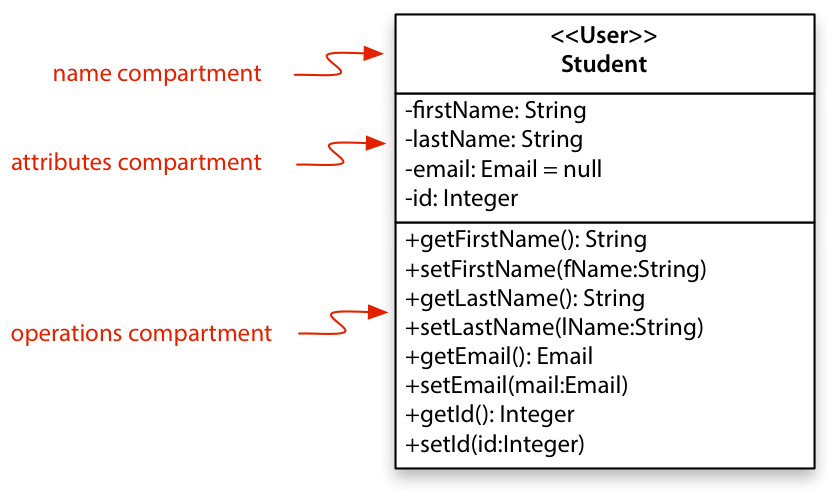
\includegraphics[height=180pt]{compartments.png}
\end{center}
  
\end{frame}

%-----------
\begin{frame}{Class Diagram:Modeling Attributes}{Attribute Visibility}
Each attribute definition must specify what other objects are allowed to see the attribute -- that is its visibility. 
Visibility is defined as follows:
    \begin{itemize}
         \item Public (+) visibility allows access to objects of all other classes.
         \item Private (-) visibility limits access to within the class itself. For example, only
operations of the class have access to a private attribute.
         \item Protected (\#) visibility allows access by subclasses. In the case of generalizations 
                   (inheritance), subclasses must have access to the attributes and operations of the superclass or 
                   they cannot be inherited.
         \item Package (\textasciitilde) visibility allows access to other objects in the same package.
   \end{itemize}
\end{frame}

%-----------
\begin{frame}{Class Diagram:Modeling Attributes}{Attribute Specification}

      \begin{tabular}{p{4.5cm}p{6.5cm}}
        \toprule
        \textbf{Attribute Element Description} & \textbf{Attribute Element Example}  \\
        \midrule
	\scriptsize Create an attribute name & \scriptsize company\\
	\scriptsize Add the attribute data type & \scriptsize company:character \\
	\scriptsize Add the attribute’s default value, if any & \scriptsize company:character = spaces \\
	\scriptsize Set the constraints on the attribute value. For this example, first identify the field length. &  
          \scriptsize         company:character = spaces \{1 to 30 characters\} \\
	\scriptsize Next identify the types of data that can be used in the attribute. Add this information within the brackets. & 
        \scriptsize    company:character = spaces \{1 to 30 characters including alphabetic, spaces, and punctuation 
                characters; no special characters allowed\} \\
	\scriptsize Set the attribute visibility (designate private visibility with a minus (-) sign in front of the attribute). 
        &\scriptsize  - company:character = spaces \{1 to 30 characters including alphabetic, spaces, and punctuation characters; 
                 no special characters allowed\} \\

        \bottomrule

      \end{tabular}
\end{frame}

%-----------
\begin{frame}{Class Diagram: Operations}
    \begin{itemize}
	\item Operation name: Required. The combination of name and parameters does need to be unique within a class.
	\item Arguments/parameters: Each argument requires an identifier and a data type. 
	\item Return data type: Required for a return value, but return values are optional. 
	\item Visibility (+, -, \#, \textasciitilde): Required before code generation. 
	\item Class level operation (underlined operation declaration): Optional. In Java: static methods.
	\item Argument name: Required for each parameter, but parameters are optional. Any number of arguments is allowed.
	\item Argument data type: Required for each parameter, but parameters are optional.
   \end{itemize}
\end{frame}

%--------
\begin{frame}{Class Diagram: Associations}
\begin{center}
  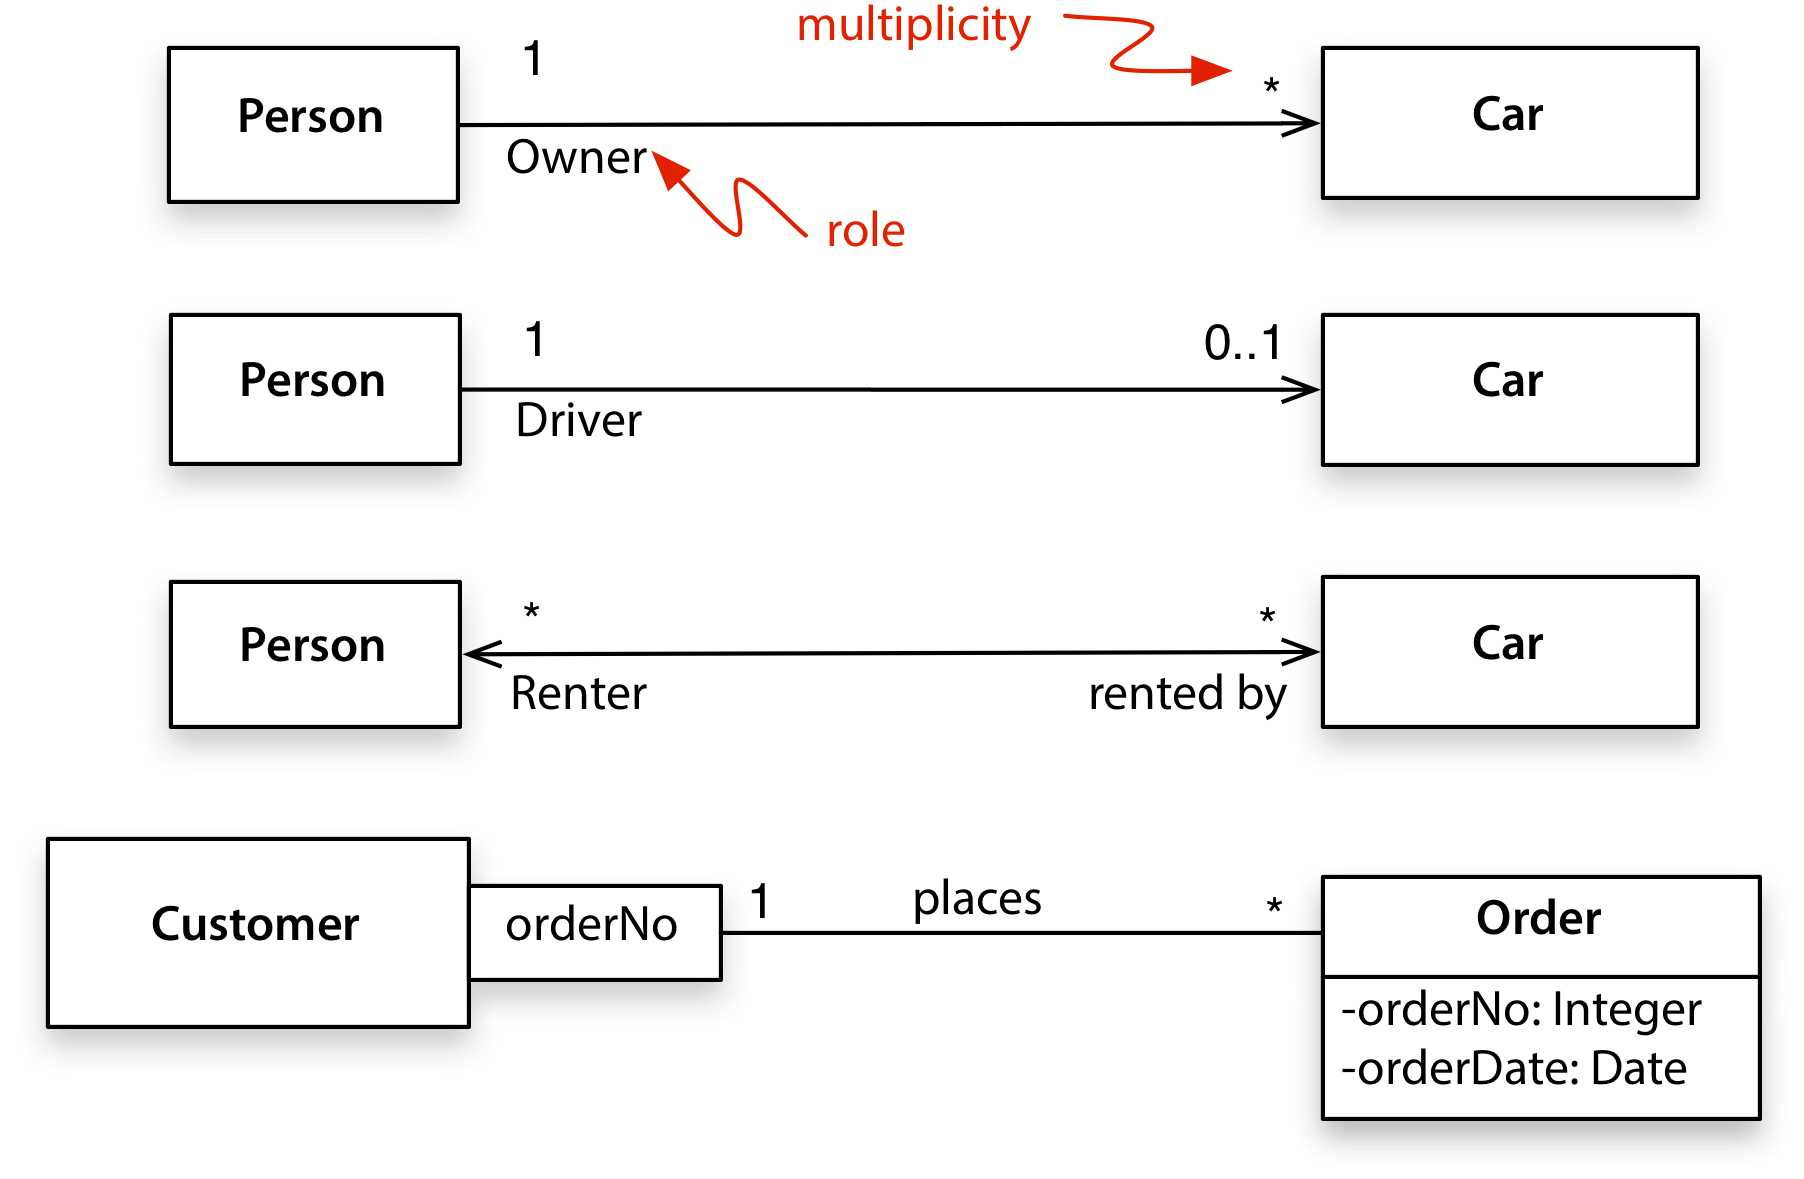
\includegraphics[scale=0.6]{associations.png}
\end{center}
  
\end{frame}

%--------
\begin{frame}{Class Diagram: Aggregation and Composition}
\begin{center}
  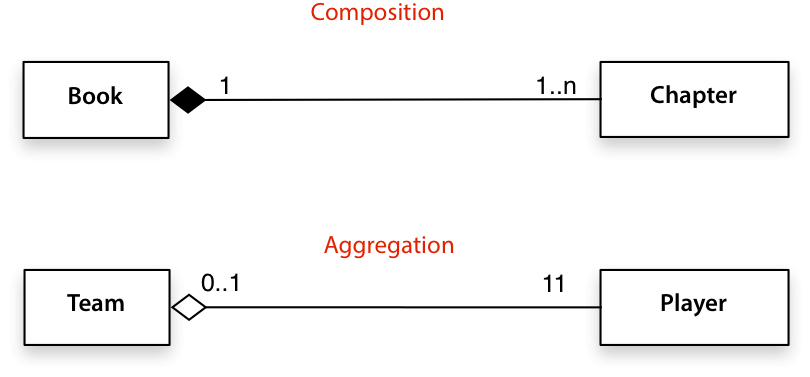
\includegraphics[scale=0.6]{aggregation.png}
\end{center}

\end{frame}

%--------
\begin{frame}{Class Diagram: Generalization}
\begin{center}
  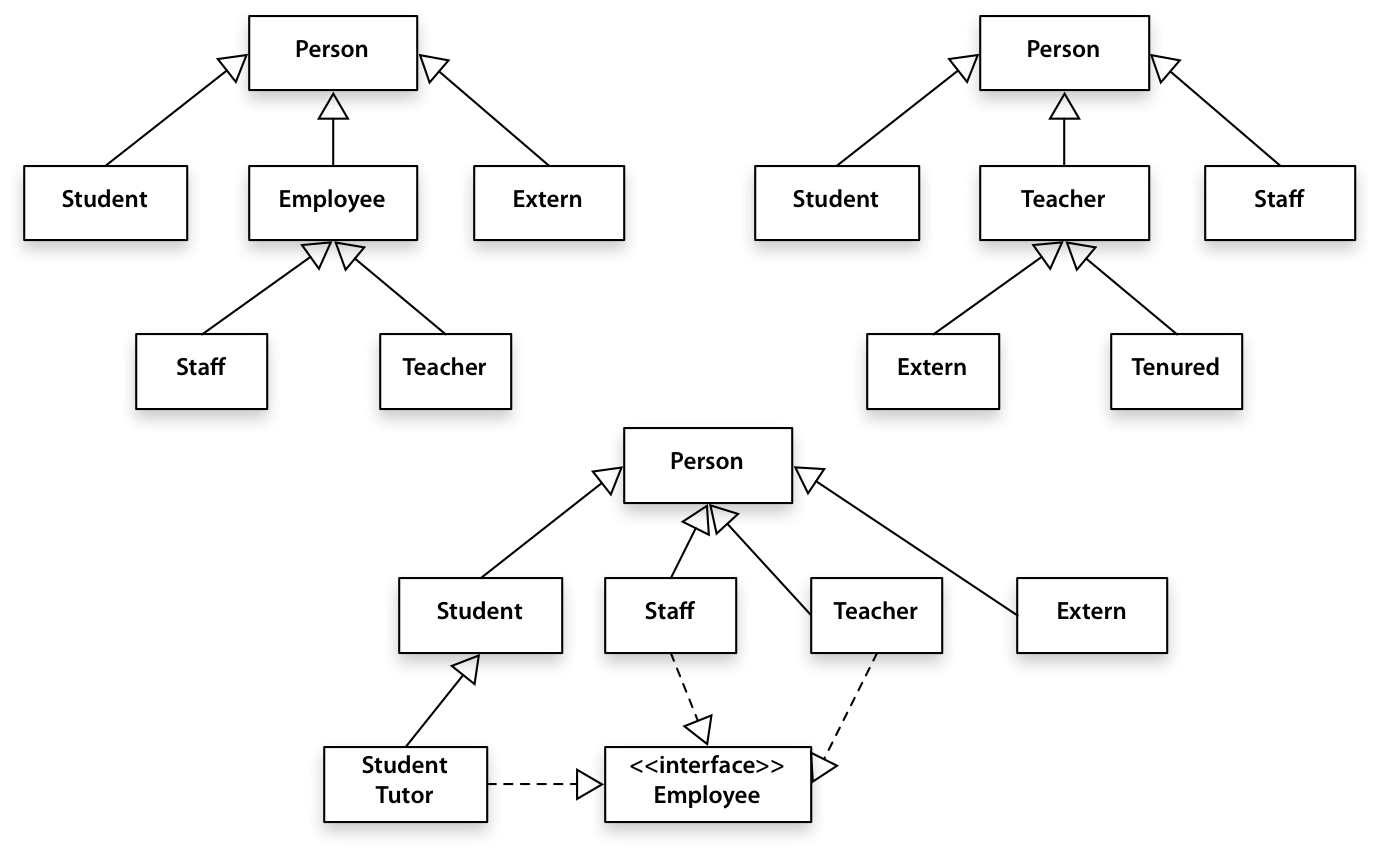
\includegraphics[height=190pt]{generalization.png}
\end{center}

\end{frame}

%***********************
% TODO more UML examples
%***********************
%
\begin{frame}{Architectural Objectives}
	The system to be designed must be
       \begin{itemize}
           \item correct
           \item extensible
           \item understandable
       \end{itemize}
	To that end we use object oriented design principles
\end{frame}

\begin{frame}{Principles of Object Oriented Design}
   \begin{block}{Principles for Single Class Design}
       \begin{itemize}
           \item Encapsulation, abstraction, and information hiding
           \item Separation of concerns and the single-responsibility principle
           \item Interface segregation principle
   \end{itemize}
   \end{block}
   \begin{block}{Principles for Design of Class Cooperation}
       \begin{itemize}
           \item Loose Coupling
           \item Liskov substitution principle
           \item Design by contract
           \item Open-close principle
           \item Dependency inversion principle
   \end{itemize}
\end{block}


\end{frame}

\subsection{Correctness, Extensibility, and Understandibility}
\subsubsection{Correctness}
\subsubsection{Extensibility}
\subsubsection{Understandibility}

\subsection{Encapsulation, abstraction, and information hiding}
\subsection{Separation of concerns and the single-responsibility principle}
\subsection{Interface segregation principle}
\subsection{Loose Coupling}
\subsection{Liskov substitution principle}
\subsection{Design by contract}
\subsection{Open-close principle}
\subsection{Dependency inversion principle}




